% Options for packages loaded elsewhere
\PassOptionsToPackage{unicode}{hyperref}
\PassOptionsToPackage{hyphens}{url}
\PassOptionsToPackage{dvipsnames,svgnames,x11names}{xcolor}
%
\documentclass[
  letterpaper,
  DIV=11,
  numbers=noendperiod]{scrartcl}

\usepackage{amsmath,amssymb}
\usepackage{lmodern}
\usepackage{setspace}
\usepackage{iftex}
\ifPDFTeX
  \usepackage[T1]{fontenc}
  \usepackage[utf8]{inputenc}
  \usepackage{textcomp} % provide euro and other symbols
\else % if luatex or xetex
  \usepackage{unicode-math}
  \defaultfontfeatures{Scale=MatchLowercase}
  \defaultfontfeatures[\rmfamily]{Ligatures=TeX,Scale=1}
\fi
% Use upquote if available, for straight quotes in verbatim environments
\IfFileExists{upquote.sty}{\usepackage{upquote}}{}
\IfFileExists{microtype.sty}{% use microtype if available
  \usepackage[]{microtype}
  \UseMicrotypeSet[protrusion]{basicmath} % disable protrusion for tt fonts
}{}
\makeatletter
\@ifundefined{KOMAClassName}{% if non-KOMA class
  \IfFileExists{parskip.sty}{%
    \usepackage{parskip}
  }{% else
    \setlength{\parindent}{0pt}
    \setlength{\parskip}{6pt plus 2pt minus 1pt}}
}{% if KOMA class
  \KOMAoptions{parskip=half}}
\makeatother
\usepackage{xcolor}
\usepackage[top=30mm,left=20mm,heightrounded]{geometry}
\setlength{\emergencystretch}{3em} % prevent overfull lines
\setcounter{secnumdepth}{5}
% Make \paragraph and \subparagraph free-standing
\ifx\paragraph\undefined\else
  \let\oldparagraph\paragraph
  \renewcommand{\paragraph}[1]{\oldparagraph{#1}\mbox{}}
\fi
\ifx\subparagraph\undefined\else
  \let\oldsubparagraph\subparagraph
  \renewcommand{\subparagraph}[1]{\oldsubparagraph{#1}\mbox{}}
\fi


\providecommand{\tightlist}{%
  \setlength{\itemsep}{0pt}\setlength{\parskip}{0pt}}\usepackage{longtable,booktabs,array}
\usepackage{calc} % for calculating minipage widths
% Correct order of tables after \paragraph or \subparagraph
\usepackage{etoolbox}
\makeatletter
\patchcmd\longtable{\par}{\if@noskipsec\mbox{}\fi\par}{}{}
\makeatother
% Allow footnotes in longtable head/foot
\IfFileExists{footnotehyper.sty}{\usepackage{footnotehyper}}{\usepackage{footnote}}
\makesavenoteenv{longtable}
\usepackage{graphicx}
\makeatletter
\def\maxwidth{\ifdim\Gin@nat@width>\linewidth\linewidth\else\Gin@nat@width\fi}
\def\maxheight{\ifdim\Gin@nat@height>\textheight\textheight\else\Gin@nat@height\fi}
\makeatother
% Scale images if necessary, so that they will not overflow the page
% margins by default, and it is still possible to overwrite the defaults
% using explicit options in \includegraphics[width, height, ...]{}
\setkeys{Gin}{width=\maxwidth,height=\maxheight,keepaspectratio}
% Set default figure placement to htbp
\makeatletter
\def\fps@figure{htbp}
\makeatother
\newlength{\cslhangindent}
\setlength{\cslhangindent}{1.5em}
\newlength{\csllabelwidth}
\setlength{\csllabelwidth}{3em}
\newlength{\cslentryspacingunit} % times entry-spacing
\setlength{\cslentryspacingunit}{\parskip}
\newenvironment{CSLReferences}[2] % #1 hanging-ident, #2 entry spacing
 {% don't indent paragraphs
  \setlength{\parindent}{0pt}
  % turn on hanging indent if param 1 is 1
  \ifodd #1
  \let\oldpar\par
  \def\par{\hangindent=\cslhangindent\oldpar}
  \fi
  % set entry spacing
  \setlength{\parskip}{#2\cslentryspacingunit}
 }%
 {}
\usepackage{calc}
\newcommand{\CSLBlock}[1]{#1\hfill\break}
\newcommand{\CSLLeftMargin}[1]{\parbox[t]{\csllabelwidth}{#1}}
\newcommand{\CSLRightInline}[1]{\parbox[t]{\linewidth - \csllabelwidth}{#1}\break}
\newcommand{\CSLIndent}[1]{\hspace{\cslhangindent}#1}

\usepackage{amsmath}
\usepackage{booktabs}
\usepackage{caption}
\usepackage{longtable}
\KOMAoption{captions}{tableheading}
\makeatletter
\makeatother
\makeatletter
\makeatother
\makeatletter
\@ifpackageloaded{caption}{}{\usepackage{caption}}
\AtBeginDocument{%
\ifdefined\contentsname
  \renewcommand*\contentsname{Table of contents}
\else
  \newcommand\contentsname{Table of contents}
\fi
\ifdefined\listfigurename
  \renewcommand*\listfigurename{List of Figures}
\else
  \newcommand\listfigurename{List of Figures}
\fi
\ifdefined\listtablename
  \renewcommand*\listtablename{List of Tables}
\else
  \newcommand\listtablename{List of Tables}
\fi
\ifdefined\figurename
  \renewcommand*\figurename{Figure}
\else
  \newcommand\figurename{Figure}
\fi
\ifdefined\tablename
  \renewcommand*\tablename{Table}
\else
  \newcommand\tablename{Table}
\fi
}
\@ifpackageloaded{float}{}{\usepackage{float}}
\floatstyle{ruled}
\@ifundefined{c@chapter}{\newfloat{codelisting}{h}{lop}}{\newfloat{codelisting}{h}{lop}[chapter]}
\floatname{codelisting}{Listing}
\newcommand*\listoflistings{\listof{codelisting}{List of Listings}}
\makeatother
\makeatletter
\@ifpackageloaded{caption}{}{\usepackage{caption}}
\@ifpackageloaded{subcaption}{}{\usepackage{subcaption}}
\makeatother
\makeatletter
\@ifpackageloaded{tcolorbox}{}{\usepackage[many]{tcolorbox}}
\makeatother
\makeatletter
\@ifundefined{shadecolor}{\definecolor{shadecolor}{rgb}{.97, .97, .97}}
\makeatother
\makeatletter
\makeatother
\ifLuaTeX
  \usepackage{selnolig}  % disable illegal ligatures
\fi
\IfFileExists{bookmark.sty}{\usepackage{bookmark}}{\usepackage{hyperref}}
\IfFileExists{xurl.sty}{\usepackage{xurl}}{} % add URL line breaks if available
\urlstyle{same} % disable monospaced font for URLs
\hypersetup{
  pdftitle={The role of cross-linguistic lexical similarity on bilingual word acquisition},
  pdfauthor={Gonzalo Garcia-Castro; Daniela S. Ávila-Varela; Ignacio Castillejo; Núria Sebastian-Galles},
  pdfkeywords={lexical acquisition, vocabulary, bilingualism},
  colorlinks=true,
  linkcolor={blue},
  filecolor={Maroon},
  citecolor={Blue},
  urlcolor={Blue},
  pdfcreator={LaTeX via pandoc}}

\title{The role of cross-linguistic lexical similarity on bilingual word
acquisition\thanks{This research was supported by grants from the
Spanish Ministerio de Ciencia, Innovación y Universidades
(PGC2018-101831-B-I00 and PRE2019-088165), and the Catalan Government
{[}ICREA (Catalan Institution for Research and Advanced Studies)
Academia 2019 award{]}. Gonzalo Garcia-Castro was supported by a
fellowship of the Spanish Ministerio de Ciencia, Innovación y
Universidades (FPI 2019). The authors declare no conflicts of interest
with regard to the funding source of this study. We are grateful to
Chiara Santolin, Alicia Franco-Martínez, Cristina Rodríguez-Prada, and
Ege E. Özer for their help-ful feedback. We thank Xavier Mayoral, Silvia
Blanch, and Cristina Cuadrado for their technical support. We also thank
Cristina Dominguez and Katia Pistrin for their efforts in recruiting
infants. We would like to thank the clinics Quirón and Sagrada Familia
that allowed us to recruit participants in their premises. We also thank
all families and infants who participated in the experiments. Data
collection was half-way when the COVID-19 pandemic started. We would
like to pay special tribute to the families that collaborated with us
under these difficult circumstances.}}
\author{Gonzalo Garcia-Castro \and Daniela S. Ávila-Varela \and Ignacio
Castillejo \and Núria Sebastian-Galles}
\date{}

\begin{document}
\maketitle
\ifdefined\Shaded\renewenvironment{Shaded}{\begin{tcolorbox}[interior hidden, boxrule=0pt, borderline west={3pt}{0pt}{shadecolor}, breakable, enhanced, sharp corners, frame hidden]}{\end{tcolorbox}}\fi

\setstretch{1.25}
\hypertarget{sec-introduction}{%
\section{Introduction}\label{sec-introduction}}

\hypertarget{word-acquisition-during-toddlerhood-the-effect-of-language-experience}{%
\subsection{Word acquisition during toddlerhood: the effect of language
experience}\label{word-acquisition-during-toddlerhood-the-effect-of-language-experience}}

The foundations of word learning are in place early in age: before the
end of their first year of life infants start directing their gaze to
some objects when hearing their labels, according to both experimental
data (Bergelson \& Swingley, 2012, 2015; Jusczyk \& Aslin, 1995; Tincoff
\& Jusczyk, 1999) and parental reports (e.g., Fenson et al., 2007).
During the last half of their second year, they acquire new words at an
increasingly fast rate (Bergelson, 2020; Bloom, 2002; Fenson et al.,
1994; Goldfield \& Reznick, 1990; Mayor \& Plunkett, 2011). These early
stages of lexical acquisition are characterised by substantial variation
across children, reflected, for instance, on the variation on the number
of words they know (i.e.~vocabulary size, Fenson et al., 1994; Frank et
al., 2021) or on the proportion of those words that fall into the
category of nouns, as opposed to verbs, adjectives, or function words
Bates et al. (1994).

Despite this variability, children's trajectories of vocabulary growth
seem quite stable across languages. Tardif et al. (2008) collected data
about the first ten words acquired by 10 to 16 month-old infants living
in the United States, Hong Kong, and Beijing. Since birth, these infants
had been learning English, Cantonese and Mandarin, respectively. The
authors found a common pattern across the three groups: their first ten
words referred to roughly the same concepts, namely relatives/caretakers
(\emph{daddy}, \emph{mommy}), social routines (\emph{bye}, \emph{uh-oh})
or animals (\emph{woof-woof}). These results were later extended by
Frank et al. (2021) to a wider diversity languages, also reporting that
such cross-language commonalities are stronger at earlier stages of
lexical acquisition, compared to later stages. Most of the literature on
early word acquisition, however, has been conducted on monolingual
children, and neglects the problem of how bilinguals--who represent a
substantial proportion of the population in most societies--acquire
words at early ages.

Previous findings point to bilingual toddlers knowing, on average, less
words in each of their languages than monolinguals, but also to both
groups knowing a similar amount of words when the two languages are
aggregated. For example, Hoff et al. (2012) found that English-Spanish
bilingual toddlers in South Florida knew less words in English than
monolinguals, who only learnt English. Both groups knew a similar total
amount of words when both English and Spanish vocabularies were counted
together, highlighting the importance of collecting data on both
languages when assessing bilinguals' communicative development. Other
studies have provided converging evidence that bilinguals know a
similar--or even larger--number of words than monolinguals, only when
the languages are aggregated (Gonzalez-Barrero et al., 2020; Oller \&
Eilers, 2002; J. Patterson et al., 2004; J. L. Patterson, 2004; Pearson
et al., 1993; Pearson \& Fernández, 1994; Petitto et al., 2001; Smithson
et al., 2014). While these studies have mostly relied on samples of
bilingual children learning two relatively distant languages, as it is
the case of English and Spanish, it is unclear whether children learning
typologically more similar languages also know less words in each of
their languages than monolinguals. What role could linguistic distance
play during early vocabulary growth?

\hypertarget{language-distance-as-a-mediator-of-bilingual-vocabulary-growth}{%
\subsection{Language distance as a mediator of bilingual vocabulary
growth}\label{language-distance-as-a-mediator-of-bilingual-vocabulary-growth}}

For a given set of concepts, bilingual children may be exposed to two
distinct sets of word-forms--one in each language. Depending on the
linguistic distance between both languages, the two sets of words may
overlap in varying degrees. Particularly, when both languages are
typologically close, like Spanish and Catalan (both Roman languages),
they are more likely to share a large amount of cognates (i.e.,
form-similar translation equivalents) than two linguistically distant
languages, like Spanish and English (one Roman, the other Germanic). For
instance, in the presence of a door, a Spanish-Italian (or a
Spanish-Catalan) bilingual might hear \emph{puerta} and \emph{porta}
(cognates), whereas a Spanish-English bilingual might hear \emph{puerta}
and \emph{door} (non-cognates). It could be the case that mapping two
phonologically similar labels (cognates like \emph{puerta}-\emph{porta})
onto the same referent is easier than doing the same with two
phonologically dissimilar labels (non-cognates, like \emph{puerta} and
\emph{door}). If cognates are easier to acquire than non-cognates,
bilinguals learning a pair of languages that share a high proportion of
cognates should benefit more often from this facilitation effect than
those learning a pair of languages with a lower proportion of cognates,
and should therefore show larger vocabulary sizes.

Floccia et al. (2018) provided evidence in line with this claim. The
authors collected vocabulary data on word comprehension and production
from 372 24-month-old bilingual toddlers living in the United Kingdom
who were learning English and an additional language. The additional
language was one a pool of 13 typologically diverse languages: Bengali,
Cantonese Chinese, Dutch, French, German, Greek, Hindi/Urdu, Italian,
Mandarin Chinese, Polish, Portuguese, Spanish and Welsh. The authors
calculated the average phonological similarity between the words in each
of these additional languages and their translation equivalents in
English. Phonological similarity was measured by computing the
Levenshtein distance between each cross-language pair of phonological
transcriptions. The Levenshtein distance is a metric that computes the
edit distance between two strings by counting the smallest number of
insertions, deletions and substitutions one of the strings has to go
through to become identical to the other (Levenshtein et al., 1966). The
resulting scores were then divided by the length of the longest string
to bound the similarity scores between 0 and 1, and then entered this
variable as a predictor as they modelled participants' vocabulary sizes.
Among other findings, the authors reported an increase in productive
vocabulary size in the additional language associated with an increase
in the average phonological similarity between the translation
equivalents of each language pair. For example, English-Dutch bilinguals
(22.14\% phonological similarity), were able to produce more Dutch words
than English-Mandarin bilinguals (1.97\% phonological similarity) were
able to produce in Mandarin.

\hypertarget{a-candidate-account-lexical-non-selectiviy-and-parallel-activation}{%
\subsection{A candidate account: lexical non-selectiviy and parallel
activation}\label{a-candidate-account-lexical-non-selectiviy-and-parallel-activation}}

Floccia et al.~pointed to \emph{parallel activation} as the main
phenomenon underpinning their results. The parallel activation
hypothesis suggests that bilinguals activate both languages
simultaneously during speech production or comprehension, and that this
phenomenon is the result of the activation of lexical representations in
both languages, even when only one is in use during production (Costa et
al., 2000; Hoshino \& Kroll, 2008) or comprehension (Spivey \& Marian,
1999; Thierry \& Wu, 2007). One of the clearest examples of parallel
activation was provided by Costa et al. (2000). In this study,
Catalan-Spanish monolingual and bilingual adults were asked to name
pictures of common objects in Spanish. In half of the trials, the object
labels were cognates in Spanish and Catalan (\emph{árbol}-\emph{arbre},
translations of \emph{tree}), whereas in the other half of the trials
labels were non-cognates (\emph{mesa}-\emph{taula}, translations of
\emph{table}). Bilinguals named cognate pictures faster than non-cognate
pictures, even after adjusting for the lexical frequency of the items.
Importantly, Spanish monolinguals--unfamiliar with the Catalan
translations of the Spanish words they uttered--did not show this
effect. These results suggest that bilinguals' Catalan phonology was
activated during the production of Spanish words, facilitating the
naming of cognate pictures. Several subsequent studies have also
provided similar evidence in comprehension in children (Poulin-Dubois et
al., 2013; e.g., Von Holzen \& Mani, 2012). Parallel activation is
therefore a plausible explanation for Floccia et al.'s results:
cognateness increases the amount of cross-language activation,
facilitating word acquisition, and ultimately leading to children
learning language pairs with a larger proportion of cognates are
predicted to show larger vocabulary sizes. This account is is line with
previous studies suggesting that the acquisition of new words is
facilitated by their phonological or semantic similarity with other
words, already acquired or not (Fourtassi et al., 2020; e.g., Hills et
al., 2009; Jones \& Brandt, 2019; Laing, 2022). Importantly, bilinguals
seem to be more likely to acquire words for which their translation
equivalent has been already learnt in the other language, suggesting
that semantic similarity also facilitates word acquisition across
languages (Bilson et al., 2015).

If phonological similarity also plays a cross-language facilitation role
during word acquisition, cognate translation equivalents--which share
both semantic and phonological similarity--should be acquired earlier
that non-cognate translation equivalents--which share semantic
similarity, but not phonological similarity. Evidence supporting and
earlier age of acquisition for cognates is scarce. Bosch \& Ramon-Casas
(2014) used vocabulary parental reports (152 lexical items) from 48
Catalan-Spanish bilinguals aged 18 months, and found that cognates
represented a larger proportion of participant's vocabulary than
non-cognates. Schelletter (2002) reported a longitudinal single case of
one English-German bilingual who produced cognates earlier than
non-cognates, on average. The low sample size in these two studies makes
it challenging to draw strong conclusions about the effect of
cognateness on vocabulary growth. On the other hand, Floccia et al.'s
estimates are statically more reliable given their (much larger) sample
size, but their study was not aimed at testing the effect of cognateness
on age of acquisition directly. In their discussion the authors state
the following (pp.~70):

\begin{quote}
``This finding also provides support to the proposal that the cognate
advantage is due to cognates being acquired before non-cognates in early
childhood (Costa et al., 2016), leading to an ease of processing later
in life.''
\end{quote}

We identify two main reasons why an earlier age of acquisition for
cognates than for non-cognates is an unwarranted conclusion from Floccia
et al.'s results. First, the response variable used was the proportion
of words each participant understood and/or produced (i.e., vocabulary
size), from the list of lexical items in the vocabulary checklists. By
aggregating the responses from all items into a single datum per child,
information about the acquisition status of cognates vs.~non-cognates
was lost. Second, all participants were aged \textasciitilde24 months,
meaning that even if the unaggregated responses to individual items were
included as response variable, the possible effect of cognateness could
only be interpreted as an increase or decrease in the likelihood of
participants at such age to have acquired each item, and not as an
increase or decrease in the age of acquisition of such item.

More recently, Mitchell et al. (2022) addressed this issue overcoming
some of these pitfalls. Using a larger, longitudinal sample of 47
16-to-30 month-old French-English bilinguals living in Canada, the
authors collected data on expressive vocabulary data in both languages.
They created two lists of translation equivalents: one made of 131
cognates, and one made of 406 non-cognates. The proportion of
translation equivalents that children were reportedly able to produce
was higher in the cognate lists than in the non-cognate list across
ages, even when both lists were matched by semantic category (furniture,
animals, food were similarity represented in both lists) and age of
acquisition norms (an index of word difficulty). These findings shed
some light on the ongoing exploration of why (if at all) bilinguals'
vocabulary size grows faster when both languages are phonologically more
similar: word-forms sharing more phonemes with their translation
equivalents (i.e., cognates) seem to be acquired faster.

\hypertarget{two-competing-mechanisms-for-a-cognate-facilitation-during-word-acquisition}{%
\subsection{Two competing mechanisms for a cognate facilitation during
word
acquisition}\label{two-competing-mechanisms-for-a-cognate-facilitation-during-word-acquisition}}

As Mitchell et al. (2022) note in their discussion, the facilitative
effect of cognateness on word acquisition can be explained by at least
two alternative but arguably incompatible mechanisms. On the one hand,
cognateness might operate at the pre-lexical level as a bidirectional
facilitator of the acquisition of the two word-forms of a translation
pair: every exposure to either word-form activates the other, and
therefore strengthens the association between both word-forms and their
referent with every exposure. For instance, hearing \emph{flower} in
English might activate \emph{floeur} in French, and \emph{vice versa}.
Repeated exposure to the English or the French words eventually leads to
an earlier acquisition for both of them, as compared to non-cognate
translation equivalents like \emph{cow} and \emph{vache}, which do not
activate each other via phonological similarity. If this is the case,
then cognateness should increase the probability of acquisition of the
word-forms in both languages equally.

Another possibility is that cognateness plays a role in the acquisition
of a translation pair only when at least one of the word-forms has been
acquired. This account departs from the premise that phonological
similarity operates at the lexical level to facilitate word learning
across languages: if the child has still not formed a lexical
representation with sufficient phonological detail for one of the word
forms, the acquisition of its translation in the other language cannot
be facilitated by cognateness. This implies that, if cognateness
facilitates the acquisition of a word form, it can only do so after the
child has acquired one of the word forms of the translation pair. Given
that children are more likely to acquire words from languages to which
they are exposed more often (Cattani et al., 2014; David \& Wei, 2008;
Thordardottir et al., 2006), the acquisition of words in the language of
lower exposure should, on average, be more susceptible to the effect of
cognateness.

In line with this second hypothesis, the size of the effect of
linguistic similarity on vocabulary size that Floccia et al.~reported
was larger in the additional language (language of lower exposure)
vocabulary than in English vocabulary (language of higher exposure. Most
participants in their sample were English-dominant, meaning that their
relative amount of exposure to English was larger than in the additional
language. Therefore, participants may have, on average, learnt the
English word-form of translation equivalents earlier than the word-form
in the additional language. If this is the case, then the acquisition of
English words by English-dominant participants would rarely benefit from
their cognate status (the other word-form is not available yet), while
the acquisition of words in the additional language would benefit from
their phonological similarity with the (available) English form.

\hypertarget{the-present-study}{%
\subsection{The present study}\label{the-present-study}}

In this study, we investigated the role of cognateness on the
acquisition of translation equivalents, and if such effect is
conditional to the amount of time the child is exposed to the
corresponding language of each member of the translation pair. Using an
online vocabulary checklist--designed specifically for this study--we
collected data from a sample of children aged 10 to 35 months learning
Catalan and/or Spanish, with varying degrees of exposure to each
language. We then adopted an Bayesian item response theory (\emph{IRT})
approach to model the probability of participants being reported by
their parents to understand or understand \emph{and} say each word in
the checklist, conditional to its cognate status in Catalan and Spanish
and participants' degree of exposure to the corresponding language,
while adjusting for other indices of word difficulty--lexical frequency
(Goodman et al., 2008) and length (phonemes)-- and participant
skill--age (see Kachergis et al., 2022 for a similar approach).

\hypertarget{sec-methods}{%
\section{Methods}\label{sec-methods}}

\hypertarget{sec-participants}{%
\subsection{Participants}\label{sec-participants}}

We collected data from 422 children from the Metropolitan Area of
Barcelona between 28th October, 2019 and 12th July, 2022. All families
gave informed consent before participating and this study was approved
by the Comitè d'Ètica de la Investigació amb Medicaments (CEIm) from
Hospital del Mar (Barcelona, Spain), code XXXXXXXXX. Families from the
participant database of the Laboratori de Recerca en Infància of the
Universitat Pompeu Fabra were contacted by e-mail or phone if their
child were aged between 10 and 35 months, and had not been reported to
be exposed more than 10\% of the time to a language other than Spanish
or Catalan. Upon consent, families were sent a link to the questionnaire
via e-mail, which they filled from a computer, laptop, or mobile device
in a browser within the two week following the invitation to
participate. Table~\ref{tbl-participants-lp} summarises the distribution
of participants across ages and degrees of exposure (DoE) to Catalan.

\begin{table}

\caption{\label{tbl-participants-lp}Participant sample size by age and
degree of exposure to Catalan.}\begin{minipage}[t]{\linewidth}
\subcaption{\label{tbl-participants-lp-1}Information about DoE was provided by families before filling the
questionnaire. A 100\textbackslash\% indicated that the participant was exclusively
exposed to Catalan, and never to Spanish. A 0\textbackslash\% indicates that the
participant was not exposed to Catalan ever, and rather most of the time
to Spanish. A 50\textbackslash\% indicates that the participant was exposed to Catalan
and Spanish approximately half of the time each. The 100\textbackslash\%, 0\textbackslash\%, and
50\textbackslash\% would be traditionaly classified as Catalan monolingual, Spanish
monolingual, and Catalan-Spanish bilingual, respectively. For
illustration purposes this table, DoEs were binned into 25\textbackslash\%-wide bins,
and ages (in months) binned into 4 month-wide bins. Hyphens indicate
that no participants from that specific combination of age and DoE
filled the questionnaire. }

{\centering 

\setlength{\LTpost}{0mm}
\begin{longtable}{l|rrrrrrrr}
\tabularnewline

\toprule
\multicolumn{1}{l}{} &  & \multicolumn{7}{c}{Age (months)} \\ 
\cmidrule(lr){3-9}
\multicolumn{1}{l}{} & DoE Catalan\textsuperscript{1} & [10,14] & (14,18] & (18,22] & (22,26] & (26,30] & (30,34] & (34,36] \\ 
\midrule
 & 75-100\% & 22 & 25 & 36 & 39 & 21 & 8 & – \\ 
 & 50-75\% & 12 & 13 & 27 & 38 & 21 & 6 & 8 \\ 
 & 25-50\% & 17 & 16 & 47 & 29 & 24 & 4 & 11 \\ 
 & 0-25\% & 15 & 12 & 21 & 19 & 9 & – & – \\ 
\midrule 
\midrule 
Total & — & $66$ & $66$ & $131$ & $125$ & $75$ & $18$ & $19$ \\ 
\bottomrule
\end{longtable}
\begin{minipage}{\linewidth}
\textsuperscript{1}This proportion is complementary to the degree of exposure to Spanish, with the exception of those participants who were also exposed to a third language up to 10\% of the time\\
\end{minipage}

}

\end{minipage}%

\end{table}

We used the highest educational attainment of parents or caretakers as a
proxy of participants' socio-economic status (SES), which families
self-reported in the questionnaire by filling two items asking for the
educational attainment of each parent or caretaker, with the following
available options: \emph{No education}, \emph{Primary},
\emph{Secondary}, \emph{Complementary}, \emph{Vocational}, and
\emph{University}, in line with the current educational system in Spain.
Most families reported university studies (403, 0.9549763), followed by
families were the highest educational attainment were vocational studies
(75, 18\%), complementary studies (6, 1\%), secondary education (7, 2\%,
0\%), no formal education (2, 0\% and primary education (1,
\textless1\%).

\hypertarget{sec-questionnaire}{%
\subsection{Questionnaire}\label{sec-questionnaire}}

To collect vocabulary data from participants, we created an \emph{ad
hoc} questionnaire, MultiLex (Garcia-Castro, 2022). This questionnaire
was inspired in the MacArthur-Bates Communicative Development Inventory
(Fenson et al., 2007) and its adaptations to other languages, and was
implemented on-line using the formR platform (Arslan et al., 2020). This
questionnaire is structured in three blocks: a (1) language
questionnaire, a (2) demographic survey, and a (3) Catalan and a Spanish
vocabulary checklists. Vocabulary checklists followed a similar
structure as the Oxford Communicative Developmental Inventory (Hamilton
et al., 2000) and consisted in two lists of words: one in Catalan and
one in Spanish. The Catalan inventory contained 798 items and the
Spanish inventory contained 802. Items in one language were translation
equivalents of the items in the other language (e.g., whenever
\emph{gos} {[}dog{]} was included in the Catalan inventory, the word
\emph{perro} was included in the Spanish inventory), roughly following a
one-to-one mapping. In case two translation equivalents were possible
for a given word, both were included as separate items (e.g., Catalan
\emph{acabar} {[}\emph{to finish}{]} and Spanish \emph{acabar} and
\emph{terminar}), or merged them into a single item (e.g., Spanish
\emph{mono} {[}\emph{monkey}{]} and Catalan \emph{mono/mico}). We
included items from a diverse sample of 27 semantic/functional
categories.

For each word in the vocabulary checklists, we asked parents to report
whether their child was able to understand it, understand \emph{and} say
it, or did not understand or say it (checked out by default). Some
families filled a long version of the vocabulary checklists (803
translation equivalents; 798 items in Catalan, 802 items in Spanish),
while others filled a shorter version (\textasciitilde400 translation
equivalents, \textasciitilde400 items in Catalan, \textasciitilde400
items in Spanish). These last families were randomly allocated into one
of four different subsets of the complete list of items. These lists
were designed so that each contained a representative sub-sample of the
items from the complete list. Semantic/functional categories with less
than 16 items--thus resulting in less than four items after dividing it
in four lists--were not divided in the short version of the
questionnaire: all of their items were included in the four lists.
Another subset of items that were part of the trial lists of some
experiments in the lab were also included in all versions. For the
analyses in the present study, we considered responses to words
corresponding to nouns, verbs, and adjectives (Fourtassi et al., 2020).
We excluded multi-word items (e.g., \emph{barrita de cereales} {[}cereal
bar{]}) and items that included more than one word-form (e.g.,
\emph{mono/mico}).

\hypertarget{variables-of-interest}{%
\subsection{Variables of interest}\label{variables-of-interest}}

We extracted four variables of interest for each word-form. (1) Word
lexical frequency (\(Frequency\)): lexical frequency of the word in its
corresponding language, expressed as Zipf scores (Van Heuven et al.,
2014; Zipf, 1949). This variable ranges from 0 to 7, and follows and
approximates a normal distribution, with most values in a corpus ranging
from 3 to 5 points. Lexical frequencies were extracted from an adult
subtitle-based database: SUBTLEX-CAT (Boada et al., 2020) for Catalan
words and SUBTLEX-ESP (Cuetos et al., 2012) for Spanish words. Using
child-based estimates of lexical frequency like CHILDES was not possible
due to the low number of Catalan participants and tokens in the
available corpora. Responses to words with missing lexical frequency
score were excluded from analyses (1.22\% of the total number of items).
(2) Word length (\(Phonemes\)): number of phonemes in the phonological
transcription of the word-form in International Phonological association
format. (3) Phonological similarity (\(Levenshtein\)): normalised
Levenshtein similarity between the word-form and its translation in the
other language (Levenshtein et al., 1966). This score is calculated by
first calculating the Levenshtein distance between the two
transcriptions (number of insertions, deletions or replacements needed
for the shortest transcription to become identical to the longer
transcription), then dividing the resulting value by the length of the
longest transcription, and finally subtracting this value from 1. This
results in a proportion that indicates how much the two phonological
transcriptions of the translation equivalent are similar to each other,
ranging from 0\% (no similarity at all) to 100\% (both transcriptions
are identical) (see Floccia et al., 2018; Fourtassi et al., 2020; Laing,
2022 for similar approaches). (4) Participant age: number of months
elapsed between participants' birth date and questionnaire completion.
Finally, (5) participant degree of exposure to the words' language
(\(DoE\)): percentage of exposure to the language the word belonged to.
For example, for a participant with 90\% exposure to Catalan, and 10\%
to Spanish, the DoE of the Catalan word \emph{taula} would be 90\%, and
the DoE for the Spanish word \emph{mesa} would be 10\%.
Table~\ref{tbl-item-summary} shows a summary of the distribution of the
word-level predictors across languages in and questionnaire versions.

\hypertarget{tbl-item-summary}{}
\begin{longtable}{lrrrrrrrrrr}
\caption{\label{tbl-item-summary}Lexical properties of the word-forms and translation pairs included in
the vocabulary checklist and our analyses. We report the number of
items, mean, standard deviation (SD), and range of the lexical frequency
(epxressed in Zipf scores), length (number of phonemes) of the word
forms, and the phonological similarity (normalised Levenshtein
similarity) with their translation equivalent. Statistics are reported
separately for Catalan and Spanish, and for the different vocabulary
checklists that participants were allocated to (A, B, C, D). }\tabularnewline

\toprule
 &  & \multicolumn{3}{c}{Frequency (Zipf)} & \multicolumn{3}{c}{Length (Phonemes)} & \multicolumn{3}{c}{Phon. similarity (Levenshtein)} \\ 
\cmidrule(lr){3-5} \cmidrule(lr){6-8} \cmidrule(lr){9-11}
 & \emph{N} & Mean & \emph{SD} & Range & Mean & \emph{SD} & Range & Mean & \emph{SD} & Range \\ 
\midrule
\multicolumn{11}{l}{Catalan} \\ 
\midrule
A & 278 & $4.39$ & $0.63$ & $2.61$–$6.52$ & $5.28$ & $1.73$ & 2–14 & $37.32\%$ & $26.94\%$ & $0.00\%$–$100.00\%$ \\ 
B & 274 & $4.39$ & $0.69$ & $1.90$–$6.31$ & $5.20$ & $1.77$ & 2–14 & $35.96\%$ & $24.74\%$ & $0.00\%$–$100.00\%$ \\ 
C & 270 & $4.36$ & $0.65$ & $2.49$–$6.54$ & $5.46$ & $1.88$ & 2–14 & $36.51\%$ & $26.11\%$ & $0.00\%$–$100.00\%$ \\ 
D & 269 & $4.38$ & $0.61$ & $2.10$–$6.10$ & $5.29$ & $1.70$ & 2–14 & $36.33\%$ & $26.40\%$ & $0.00\%$–$100.00\%$ \\ 
\midrule
\multicolumn{11}{l}{Spanish} \\ 
\midrule
A & 277 & $4.25$ & $0.74$ & $2.28$–$6.76$ & $5.66$ & $1.63$ & 3–14 & $37.33\%$ & $26.89\%$ & $0.00\%$–$100.00\%$ \\ 
B & 281 & $4.28$ & $0.79$ & $2.16$–$6.14$ & $5.67$ & $1.68$ & 2–14 & $36.18\%$ & $24.95\%$ & $0.00\%$–$100.00\%$ \\ 
C & 278 & $4.24$ & $0.77$ & $1.68$–$6.26$ & $5.79$ & $1.79$ & 3–14 & $36.53\%$ & $26.24\%$ & $0.00\%$–$100.00\%$ \\ 
D & 273 & $4.24$ & $0.72$ & $1.98$–$6.14$ & $5.72$ & $1.68$ & 2–14 & $36.59\%$ & $26.55\%$ & $0.00\%$–$100.00\%$ \\ 
\bottomrule
\end{longtable}

\hypertarget{sec-analysis}{%
\subsection{Data analysis}\label{sec-analysis}}

We gathered 258,095 observations, with each observation corresponding to
a single response of one participant to a given item in the
questionnaire). These observations correspond to 395 distinct
participants (of which 343 participated once, 33 twice, 14 three times,
and 5 four times), responding to 1,199 distinct items (597 in Catalan,
602 in Spanish, 602 translation equivalents). Translation equivalents
(TEs) received a median of 236 responses (\emph{Min} = 118, \emph{Max} =
942), both languages summed together.

We modelled the probability of answering each response category
(\emph{No} \textless{} \emph{Understands} \textless{} \emph{Understands
and Says}) using a Bayesian, mixed-effects ordinal regression model (2
sampling chains with 2,000 iterations each). This model allowed us to
estimate both item and participant word-acquisition trajectories, as a
function of different fixed effects from \(Age\), \(Frequency\),
\(Phonemes\), \(DoE\), and \(Levenshtein\). We also included participant
and item random intercepts and slopes when appropriate (Barr et al.,
2013) see~\ref{sec-appendix-words}. We compared a baseline model
\(\mathcal{M}_{0}\), which only included the intercept, \(Age\),
\(Frequency\), \(Phonemes\), and \(DoE\) as predictors, with
increasingly more complex models, introducing predictors in the
following order: \(Age \times DoE\) (\(\mathcal{M}_{1}\)),
\(Levenshtein\) (\(\mathcal{M}_{2}\)), \(DoE \times Levenshtein\)
(\(\mathcal{M}_{3}\)), and finally \(Age \times Levenshtein\) and
\(Age \times DoE \times Levenshtein\) (\(\mathcal{M}_{4}\)). We compared
the predictive performance of the models using Bayesian leave-one-out
cross-validation (LOO, Vehtari et al., 2017)\footnote{Due to
  computational constraints, we performed LOO based on a random
  sub-sample of 700 samples of the posterior distribution of the fixed
  effects (Magnusson et al., 2019)}, and selected for interpretation the
one showing the best performance.

We assessed the practical relevance of the estimated regression
coefficients of the selected model by specifying a region of practical
equivalence (\emph{ROPE}, Kruschke \& Liddell, 2018) from -0.1 to +0.1
see~\ref{sec-appendix-rope}. This region indicates the range of values
that we considered as equivalent to zero. The degree of overlap between
the posterior distribution of a regression coefficient with the
\emph{ROPE} can be interpreted as support for the true parameter of the
coefficient being zero. In the results section, we report the 95\%
highest density interval (\emph{HDI}) of the posterior distribution of
each regression coefficient. This is interval contains the true value of
this coefficient with 95\% probability, given our data. We also report
the proportion of posterior samples in the 95\% \emph{HDI} that overlap
with the \emph{ROPE}, which indicates the probability that the true
value of the regression coefficient falls into the \emph{ROPE}, and
should therefore be considered equivalent to zero\footnote{For example,
  a 90\% overlap between the \emph{HDI} of the coefficients' posterior
  distribution and the \emph{ROPE} indicates that, given our data, there
  is a 90\% probability that the true value of the coefficient falls
  within the \emph{ROPE}, and is therefore equivalent to zero}.

Data processing and visualisation was done in R (R Core Team, 2020)
using the \texttt{tidyverse} family of packages (Wickham et al., 2019),
Bayesian modelling was done using the \texttt{brms} (Bürkner, 2017;
Carpenter et al., 2017), \texttt{loo} (Yao et al., 2017), and
\texttt{tidybayes} (Kay, 2021) R packages. Data and materials are
available at OSF \url{https://osf.io/hy984/}, and code is available at
GitHub \url{https://github.com/gongcastro/trajectories}.

\hypertarget{sec-results}{%
\section{Results}\label{sec-results}}

\hypertarget{sec-comparison}{%
\subsection{Model comparison and selection}\label{sec-comparison}}

The extended model (\(\mathcal{M}_{4}\)), which included the three-way
interaction between \(Age\), \(DoE\), and \(Levenshtein\) showed the
best predictive performance, with a difference in expected log-predicted
density (\emph{ELPD}) compared to the other models several times larger
than the standard error of such difference see~\ref{tbl-results-loos}.
This indicates that, given the data, the predictions of the
\(\mathcal{M}_{4}\) are confidently more accurate than those of the
other models.

\hypertarget{tbl-results-loos}{}
\setlength{\LTpost}{0mm}
\begin{longtable}{rrrrrrrrr}
\caption{\label{tbl-results-loos}Bayesian leave-one-out cross validation (LOO-CV). The predictive
accuracy of the models was compared using leave-one-out
cross-validation. The likelihood of each data point given a model fitted
without including that same observation was estimated. The resulting
likelihoods of each model were summarised as its expected log-predicted
density (ELPD), which penalises the complexity of each model. ELPD
values closer to zero indicate better predictive acuracy. We report the
ELPD, effective number of parameters (p), and information criterion (IC)
of each model along their associated standard errors (SE). The last
column indicates the difference in ELPD between each model and the model
with the best predictive accuracy (model 3). }\tabularnewline

\toprule
 & \multicolumn{2}{c}{LOOELPD} & \multicolumn{2}{c}{LOOp} & \multicolumn{2}{c}{LOOIC} & \multicolumn{2}{c}{LOOdiff} \\ 
\cmidrule(lr){2-3} \cmidrule(lr){4-5} \cmidrule(lr){6-7} \cmidrule(lr){8-9}
Model & \emph{ELPD} & \emph{SE} & \emph{p} & \emph{SE} & \emph{LOO-IC} & \emph{SE} & \emph{diff} & \emph{SE} \\ 
\midrule
4 & $-252,321.17$ & $357.98$ & $2,059.83$ & $5.72$ & $504,642.34$ & $715.96$ & $0.00$ & $0.00$ \\ 
0 & $-252,336.70$ & $356.17$ & $1,252.77$ & $3.17$ & $504,673.41$ & $712.35$ & $-15.53$ & $61.09$ \\ 
1 & $-252,346.99$ & $359.27$ & $1,720.27$ & $5.16$ & $504,693.98$ & $718.54$ & $-25.82$ & $52.40$ \\ 
3 & $-252,480.77$ & $361.35$ & $1,952.24$ & $5.38$ & $504,961.53$ & $722.70$ & $-159.60$ & $32.20$ \\ 
2 & $-253,895.47$ & $363.30$ & $2,086.79$ & $5.73$ & $507,790.94$ & $726.60$ & $-1,574.30$ & $66.98$ \\ 
\bottomrule
\end{longtable}
\begin{minipage}{\linewidth}
Pareto-\emph{k} estimates of all models were acceptable (\emph{k} \textless{} 0.5)\\
\end{minipage}

\hypertarget{sec-coefficients}{%
\subsection{Regression coefficients}\label{sec-coefficients}}

Table~\ref{tbl-results-fixed} shows the summary of the posterior
distribution of the fixed regression coefficients of the selected model.
For interpretability, we supplement the summaries of each posterior
regression coefficient with its transformation to the probability scale.
The resulting values correspond to the maximum difference in probability
of acquisition (\emph{Comprehension} or \emph{Comprehension and
Production}) that corresponds to a one standard deviation change in each
predictor\footnote{The logit and probability scales related
  non-linearly. This means that one logit difference is not necessarily
  translated to a unique value in the probability scale. For example,
  the probability of acquisition of a given word might increase in 5\%
  when age increases from 22 to 23 months, the probability of
  acquisition of the same word might only increase in 0.2\% when age
  increases from 34 to 36 months. The linear growth of the probability
  of acquisition differs along the logistic curve, and therefore
  deciding the age point at which to report the estimates of the
  regression coefficients in the probability scale is not trivial. We
  followed the suggestion by Gelman et al. (2020) and report the maximum
  value of such coefficient, which corresponds to the linear growth
  (i.e.~derivative) of the logistic curve at the age at which most
  participants were acquiring a given word. This value can be
  approximated by dividing the coefficient in the logit scale by four:
  \(\hat{\beta_j}/4\), where \(\hat{\beta_j}\) is the estimated mean of
  the posterior distribution of coefficient \(j\).}.

\hypertarget{tbl-results-fixed}{}
\begin{longtable}{lrrr}
\caption{\label{tbl-results-fixed}Posterior distribution of regression coefficients. Median: median of the
posterior distribution in the logit scale. 95\% HDI: 95\% highest
density interval (HDI) of the distribution; narrowest range of values
that contains 95\% of the distribution, and therefore is 95\% likely to
contain the true value, given the data. ROPE Prob.: percentage of the
posterior samples that fall within the region o practical equivalence
(ROPE, {[}-0.1, 0.1{]} in the logit scale); posterior probability of the
true value of the parameter being equivalent to zero. }\tabularnewline

\toprule
Parameter & Median & 95\% \emph{HDI} & \emph{ROPE} prob. \\ 
\midrule
Intercept (Comprehension and Production at 22 months) & $-0.92$ & [$-1.04$, $-0.80$] & $0.00\%$ \\ 
Intercept (Comprehension at 22 months) & $1.55$ & [$1.43$, $1.67$] & $0.00\%$ \\ 
Age (+1 SD, 5.72 months) & $1.34$ & [$1.19$, $1.48$] & $0.00\%$ \\ 
DoE (+1 SD, 30\%) & $0.40$ & [$0.27$, $0.51$] & $0.00\%$ \\ 
Levenshtein (+1 SD, 26\%) & $0.03$ & [$-0.09$, $0.13$] & $92.39\%$ \\ 
Frequency (+1 SD, 0.7 Zipf) & $0.15$ & [$0.08$, $0.23$] & $7.03\%$ \\ 
Phonemes (+1 SD, 1.75 phonemes) & $-0.15$ & [$-0.23$, $-0.08$] & $6.89\%$ \\ 
Age × DoE & $0.12$ & [$-0.01$, $0.24$] & $35.16\%$ \\ 
Age × Levenshtein & $0.05$ & [$0.01$, $0.09$] & $100.00\%$ \\ 
DoE × Levenshtein & $-0.14$ & [$-0.18$, $-0.11$] & $0.00\%$ \\ 
Age × DoE × Levenshtein & $-0.05$ & [$-0.08$, $-0.01$] & $100.00\%$ \\ 
\bottomrule
\end{longtable}

\(Age\) was the predictor with the largest effect on the probability of
acquisition (\(\beta\) = 1.34, 95\% \emph{HDI} = {[}1.19, 1.48{]}): at
the steepest point of the acquisition trajectory of an average
translation equivalent, the probability of acquisition increased 5.84\%
every month. Lexical frequency (\(Frequency\)) had a small, positive,
but inconclusive on the probability of acquisition substantially,
(\(\beta\) = 15.41\%, 95\% \emph{HDI} = {[}7.59\%, 23.08\%{]}): 7.03\%
of its posterior samples overlapped with the \emph{ROPE.} The 95\%
\emph{HDI} of the regression coefficient of the number of phonemes
(\(Phonemes\)) did exclude the \emph{ROPE}, although not by much: 6.89\%
of its posterior samples fell within the \emph{ROPE}. This suggests that
the number of phonemes in the word form had a small effect on the
probability of acquisition (\(\beta\) = -15.10\%, 95\% \emph{HDI} =
{[}-22.70\%, -7.95\%{]}). For every increase in phoneme length, the
probability of acquisition decreased in -2.16\%.

The degree of exposure to the language (\(DoE\)) had a strong effect on
the probability of acquisition (\(\beta\) = 40.00\%, 95\% \emph{HDI} =
{[}27.03\%, 50.78\%{]}). All of the posterior samples of his regression
excluded the \emph{ROPE}. The impact of this predictor on the
probability of acquisition was positive: for every 10\% increase in
exposure to the language the word belongs to, the participant was
13.34\% more likely to acquire it. The effect of phonological similarity
by itself (as indicated by the regression coefficient of the main effect
of \(Levenshtein\)) was equivalent to zero (\(\beta\) = 3.12\%, 95\%
\emph{HDI} = {[}-8.89\%, 13.19\%{]}), as 92.39\% of the posterior
samples of its regression coefficient fell into the \emph{ROPE}.
However, the 95\% \emph{HDI} of the regression coefficient of the
\(Doe \times Levenshtein\) interaction excluded the \emph{ROPE} entirely
(\(\beta\) = -14.46\%, 95\% \emph{HDI} = {[}-17.79\%, -11.10\%{]}),
suggesting that the effect of phonological similarity on a word's
probability of acquisition changed depending on participants' exposure
to the language it belonged to. Follow up analyses on this interaction
(see Figure~\ref{fig-results-marginal}) showed that, when exposure to
the language was low (e.g., 10\%), phonological similarity increased the
probability of acquisition substantially. This effect was negligible
when exposure to both languages was balanced (e.g.~50-50\%). Finally,
when exposure to the language was high (e.g., 90\%), this effect was
very close to zero, although with different direction, with phonological
less similar translation equivalents being more likely to be acquired
than phonologically more similar ones.

The 95\% \emph{HDI} of the regression coefficient of the
\(Age \times DoE\) interaction did not exclude the \emph{ROPE}
(\(\beta\) = 12.32\%, 95\% \emph{HDI} = {[}-1.48\%, 24.19\%{]}): 35.16\%
of its posterior samples fell within the \emph{ROPE}. This shows that
the effect of the degree of exposure on the speed at which participants
acquired word across ages was inconclusive. Give our data, it is
difficult to tell whether this \emph{DoE} increased or decreased the
slope of the words' acquisition trajectories. The 95\% \emph{HDI} of the
regression coefficient of the \(Age \times Levenshtein\) interaction
overlapped completely with the \emph{ROPE} (\(\beta\) = 4.76\%, 95\%
\emph{HDI} = {[}0.83\%, 8.77\%{]}), indicating that phonological
similarity did not speed-up the acquisition trajectories of the words
across ages. Finally, the 95\% \emph{HDI} of the regression coefficient
of the \(Age \times DoE \times Levenshtein\) interaction also overlapped
completely with the \emph{ROPE} (\(\beta\) = , 95\% \emph{HDI} =
{[}-7.56\%, -1.23\%{]}), suggesting that the impact of the degree of
exposure to the language on the effect of phonological similarity did
not differ substantially across ages.

\begin{figure}

{\centering 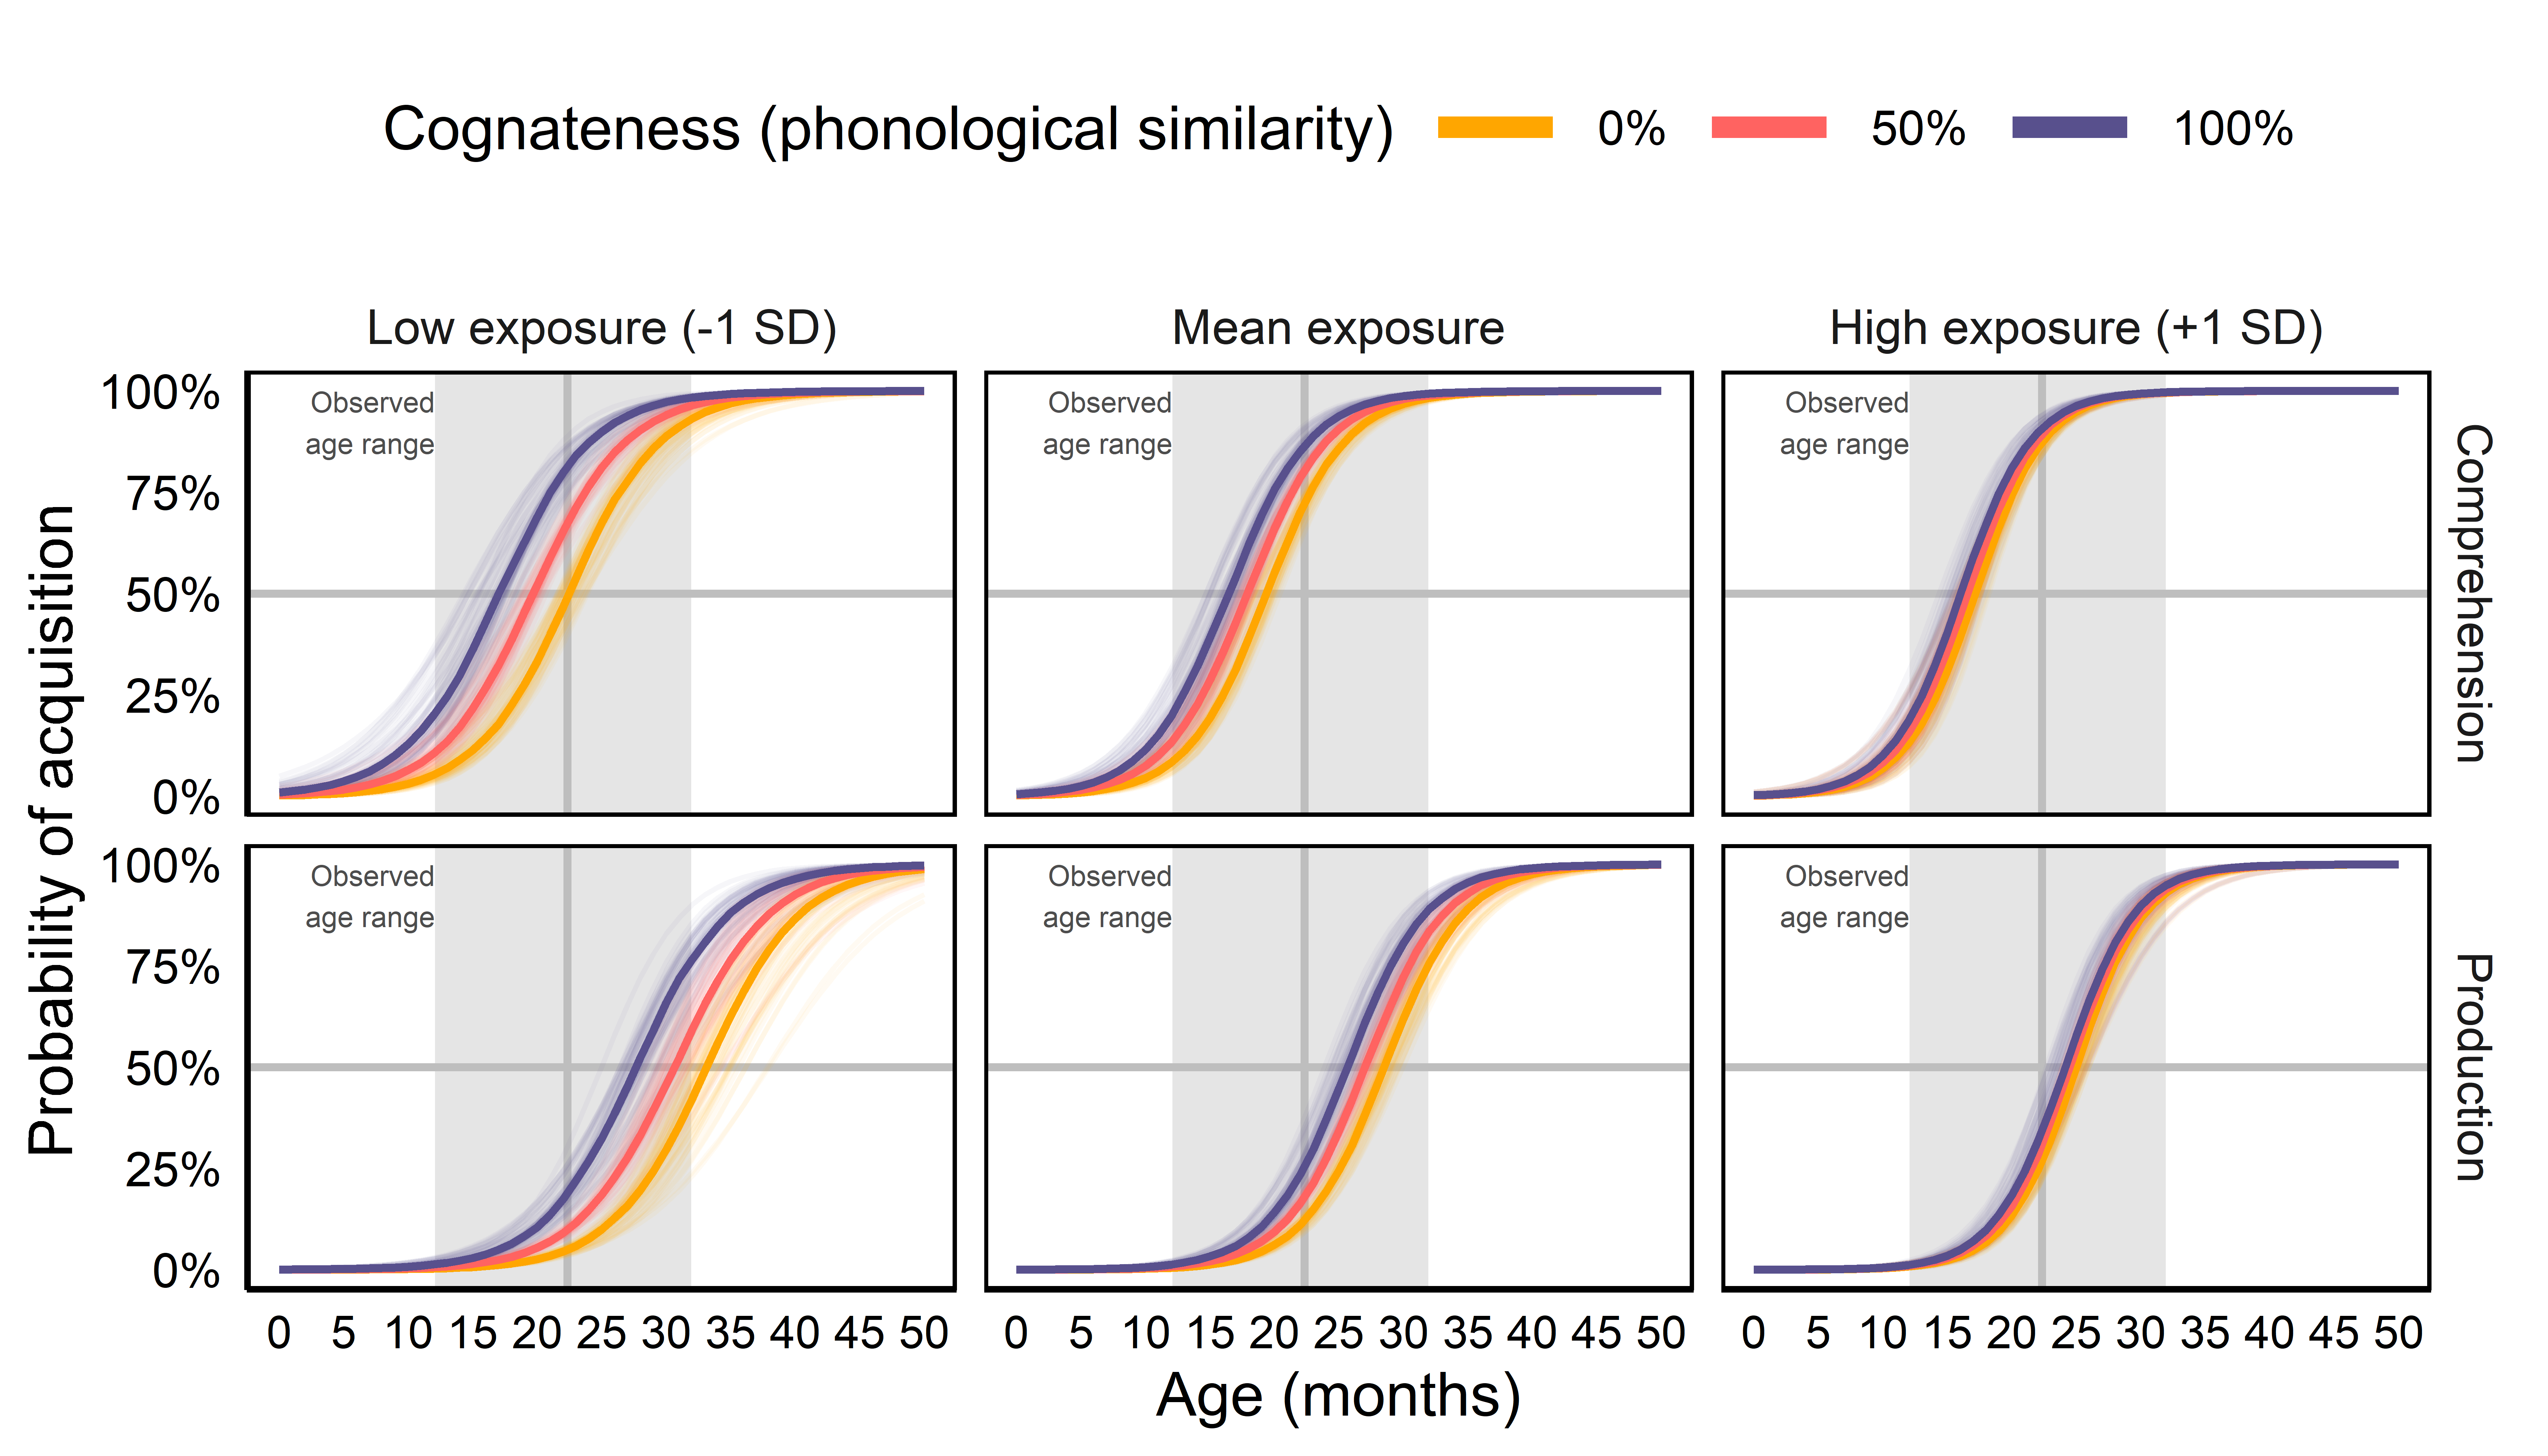
\includegraphics[width=1\textwidth,height=\textheight]{manuscript_files/figure-pdf/fig-results-marginal-1.pdf}

}

\caption{\label{fig-results-marginal}Expected posterior predictions.
Posterior poreditions for the extended model were generated by computing
the probability acquisition that resulted from feeding the equation of
the regression model with values of the posterior distribution of each
coefficient. These values correspond to the 4,000 samples of the
posterior distribution that were drawn during the MCMC estimation of the
model. Therefore, we generated 4,000 predictions for a series of
combination of levels of interest. Each line and interval and in the
figure summarises the mean and 95\% \emph{HDI} of each combination of
levels. The X-axis indicates the age (in months) for which the
prediction is generated. The Y-axis indicates the predicted probability
of acquisition (\emph{Comprehension} or \emph{Comprehension and
Production}). Different colours indicate different levels of
phonological similarity (as indicated by the Levenshtein similarity
between pairs of translation equivalents). Finally, predictions are
presented separately for different degrees of exposure (\emph{DoE}):
little exposure to the language (10\% DoE, traditionally classified as
monolingual), balanced exposure to both languages (50\%, traditionally
classified as bilingual), and high exposure to the language (90\%,
traditionally classified as monolingual). Predictions for
\emph{Comprehension} are show on top and predictions for
\emph{Comprehension and Production} are shown on the bottom.}

\end{figure}

\hypertarget{sec-discussion}{%
\section{Discussion}\label{sec-discussion}}

\hypertarget{summary-of-the-study}{%
\subsection{Summary of the study}\label{summary-of-the-study}}

\begin{itemize}
\tightlist
\item
  This study explored how word acquisition is affected by cognateness in
  bilingual toddlers.
\item
  We collected vocabulary data from children learning Catalan and/or
  Spanish in differing degrees of exposure to each, and then measured
  the probability of each word being acquired at different ages as a
  function of (1) participants' exposure to the language it belongs to,
  and (2) its phonological similarity with its translation equivalent in
  the other language.
\item
  Using item response theory (\emph{IRT}), we built an Bayesian model
  that estimated the effect of both predictors and their interaction,
  adjusting for other variables known to be relevant for the acquisition
  of words: participants' age, lexical frequency, and word length in
  phonemes.
\end{itemize}

\hypertarget{summary-of-results-and-contrast-with-the-literature}{%
\subsection{Summary of results and contrast with the
literature}\label{summary-of-results-and-contrast-with-the-literature}}

\begin{itemize}
\tightlist
\item
  We replicated effects reported in previous studies, such as age being
  the most determinant predictor of word acquisition, followed by
  exposure to the language, that frequent words are acquired earlier,
  and that word length predicts a later age of acquisition.
\item
  Regarding our hypotheses, we found strong evidence for a two-way
  interaction between language exposure and phonological similarity:
  participants were more likely to acquire word-forms from cognate
  translation equivalents than from non-cognate translation equivalents,
  but only when their exposure to the language of such word-form was
  low.
\item
  Our results converge with previous findings indicating that
  phonological similarity between translation equivalents plays a
  facilitation role in word acquisition, but suggest that this effect is
  mostly, or only present in participants' language of lower exposure.
\end{itemize}

\hypertarget{mechanistic-explanations}{%
\subsection{Mechanistic explanations}\label{mechanistic-explanations}}

\begin{itemize}
\tightlist
\item
  These findings support the hypothesis that the cognate facilitation
  effect on word acquisition is more likely to play such role
  \emph{after} one of the word-forms of the translation equivalent has
  been acquired in one of the languages, as opposed to taking place
  before any of the forms has been acquired, by promoting their
  acquisition though cross-language activation at the sub-lexical,
  phonological level.
\item
  In line with the first hypothesis, words in the language of higher
  exposure are likely to be acquired earlier than those in the language
  of lower exposure, and also showed a larger effect facilitation effect
  of cognateness.
\item
  This suggests that cognateness might have played a larger role during
  the acquisition of words from the language of lower exposure than from
  the language of higher exposure in bilinguals
\end{itemize}

\hypertarget{limitations}{%
\subsection{Limitations}\label{limitations}}

\begin{itemize}
\tightlist
\item
  These results come from a particular population of bilingual toddlers
  that learn two very similar languages--Catalan and Spanish--and are
  therefore exposed to many cognates. Our results might not generalise
  to other groups of bilinguals learning two less similar languages.
\item
  {[}To be discussed{]}
\end{itemize}

\hypertarget{further-steps}{%
\subsection{Further steps}\label{further-steps}}

\begin{itemize}
\tightlist
\item
  {[}To be discussed{]}
\end{itemize}

\hypertarget{sec-references}{%
\section{References}\label{sec-references}}

\hypertarget{refs}{}
\begin{CSLReferences}{1}{0}
\leavevmode\vadjust pre{\hypertarget{ref-arslan2020formr}{}}%
Arslan, R. C., Walther, M. P., \& Tata, C. S. (2020). Formr: A study
framework allowing for automated feedback generation and complex
longitudinal experience-sampling studies using r. \emph{Behavior
Research Methods}, \emph{52}(1), 376--387.

\leavevmode\vadjust pre{\hypertarget{ref-barr2013random}{}}%
Barr, D. J., Levy, R., Scheepers, C., \& Tily, H. J. (2013). Random
effects structure for confirmatory hypothesis testing: Keep it maximal.
\emph{Journal of Memory and Language}, \emph{68}(3), 255--278.

\leavevmode\vadjust pre{\hypertarget{ref-bates1994developmental}{}}%
Bates, E., Marchman, V., Thal, D., Fenson, L., Dale, P., Reznick, J. S.,
Reilly, J., \& Hartung, J. (1994). Developmental and stylistic variation
in the composition of early vocabulary. \emph{Journal of Child
Language}, \emph{21}(1), 85--123.

\leavevmode\vadjust pre{\hypertarget{ref-bergelson2020comprehension}{}}%
Bergelson, E. (2020). The comprehension boost in early word learning:
Older infants are better learners. \emph{Child Development
Perspectives}, \emph{14}(3), 142--149.

\leavevmode\vadjust pre{\hypertarget{ref-bergelson2012months}{}}%
Bergelson, E., \& Swingley, D. (2012). At 6--9 months, human infants
know the meanings of many common nouns. \emph{Proceedings of the
National Academy of Sciences}, \emph{109}(9), 3253--3258.

\leavevmode\vadjust pre{\hypertarget{ref-bergelson2015early}{}}%
Bergelson, E., \& Swingley, D. (2015). Early word comprehension in
infants: Replication and extension. \emph{Language Learning and
Development}, \emph{11}(4), 369--380.

\leavevmode\vadjust pre{\hypertarget{ref-bilson2015semantic}{}}%
Bilson, S., Yoshida, H., Tran, C. D., Woods, E. A., \& Hills, T. T.
(2015). Semantic facilitation in bilingual first language acquisition.
\emph{Cognition}, \emph{140}, 122--134.

\leavevmode\vadjust pre{\hypertarget{ref-bloom2002children}{}}%
Bloom, P. (2002). \emph{How children learn the meanings of words}. MIT
press.

\leavevmode\vadjust pre{\hypertarget{ref-boada2020subtlex}{}}%
Boada, R., Guasch, M., Haro, J., Demestre, J., \& Ferré, P. (2020).
SUBTLEX-CAT: Subtitle word frequencies and contextual diversity for
catalan. \emph{Behavior Research Methods}, \emph{52}(1), 360--375.

\leavevmode\vadjust pre{\hypertarget{ref-bosch2014first}{}}%
Bosch, L., \& Ramon-Casas, M. (2014). First translation equivalents in
bilingual toddlers' expressive vocabulary: {Does} form similarity
matter? \emph{International Journal of Behavioral Development},
\emph{38}(4), 317--322. \url{https://doi.org/10.1177/0165025414532559}

\leavevmode\vadjust pre{\hypertarget{ref-burkner2017brms}{}}%
Bürkner, P.-C. (2017). Brms: An r package for bayesian multilevel models
using stan. \emph{Journal of Statistical Software}, \emph{80}(1), 1--28.

\leavevmode\vadjust pre{\hypertarget{ref-carpenter2017stan}{}}%
Carpenter, B., Gelman, A., Hoffman, M. D., Lee, D., Goodrich, B.,
Betancourt, M., Brubaker, M., Guo, J., Li, P., \& Riddell, A. (2017).
Stan: A probabilistic programming language. \emph{Journal of Statistical
Software}, \emph{76}(1), 1--32.

\leavevmode\vadjust pre{\hypertarget{ref-cattani2014much}{}}%
Cattani, A., Abbot-Smith, K., Farag, R., Krott, A., Arreckx, F., Dennis,
I., \& Floccia, C. (2014). How much exposure to english is necessary for
a bilingual toddler to perform like a monolingual peer in language
tests? \emph{International Journal of Language \& Communication
Disorders}, \emph{49}(6), 649--671.

\leavevmode\vadjust pre{\hypertarget{ref-costa2000cognate}{}}%
Costa, A., Caramazza, A., \& Sebastian-Galles, N. (2000). The cognate
facilitation effect: Implications for models of lexical access.
\emph{Journal of Experimental Psychology: Learning, Memory, and
Cognition}, \emph{26}(5), 1283.

\leavevmode\vadjust pre{\hypertarget{ref-cuetos2012subtlex}{}}%
Cuetos, F., Glez-Nosti, M., Barbón, A., \& Brysbaert, M. (2012).
SUBTLEX-ESP: Spanish word frequencies based on film subtitles.
\emph{Psicol{ó}gica}, \emph{33}(2), 133--143.

\leavevmode\vadjust pre{\hypertarget{ref-david2008individual}{}}%
David, A., \& Wei, L. (2008). Individual differences in the lexical
development of french--english bilingual children. \emph{International
Journal of Bilingual Education and Bilingualism}, \emph{11}(5),
598--618.

\leavevmode\vadjust pre{\hypertarget{ref-fenson2007macarthur}{}}%
Fenson, L. et al. (2007). \emph{MacArthur-bates communicative
development inventories}. Paul H. Brookes Publishing Company Baltimore,
MD.

\leavevmode\vadjust pre{\hypertarget{ref-fenson1994variability}{}}%
Fenson, L., Dale, P. S., Reznick, J. S., Bates, E., Thal, D. J.,
Pethick, S. J., Tomasello, M., Mervis, C. B., \& Stiles, J. (1994).
Variability in early communicative development. \emph{Monographs of the
Society for Research in Child Development}, i--185.

\leavevmode\vadjust pre{\hypertarget{ref-floccia2018introduction}{}}%
Floccia, C., Sambrook, T. D., Delle Luche, C., Kwok, R., Goslin, J.,
White, L., Cattani, A., Sullivan, E., Abbot-Smith, K., Krott, A., et al.
(2018). I: INTRODUCTION. \emph{Monographs of the Society for Research in
Child Development}, \emph{83}(1), 7--29.

\leavevmode\vadjust pre{\hypertarget{ref-fourtassi2020growth}{}}%
Fourtassi, A., Bian, Y., \& Frank, M. C. (2020). The growth of
children's semantic and phonological networks: Insight from 10
languages. \emph{Cognitive Science}, \emph{44}(7), e12847.

\leavevmode\vadjust pre{\hypertarget{ref-frank2021variability}{}}%
Frank, M. C., Braginsky, M., Yurovsky, D., \& Marchman, V. A. (2021).
\emph{Variability and consistency in early language learning: The
wordbank project}. MIT Press.

\leavevmode\vadjust pre{\hypertarget{ref-multilex}{}}%
Garcia-Castro, G. (2022). \emph{Multilex: A r package for multilingual
lexical assessment using online surveys}.
\url{https://github.com/gongcastro/multilex}

\leavevmode\vadjust pre{\hypertarget{ref-gelman2020regression}{}}%
Gelman, A., Hill, J., \& Vehtari, A. (2020). \emph{Regression and other
stories}. Cambridge University Press.

\leavevmode\vadjust pre{\hypertarget{ref-goldfield1990early}{}}%
Goldfield, B. A., \& Reznick, J. S. (1990). Early lexical acquisition:
Rate, content, and the vocabulary spurt. \emph{Journal of Child
Language}, \emph{17}(1), 171--183.

\leavevmode\vadjust pre{\hypertarget{ref-gonzalez2020bilingual}{}}%
Gonzalez-Barrero, A. M., Schott, E., \& Byers-Heinlein, K. (2020).
\emph{Bilingual adjusted vocabulary: A developmentally-informed
bilingual vocabulary measure}.

\leavevmode\vadjust pre{\hypertarget{ref-goodman2008does}{}}%
Goodman, J. C., Dale, P. S., \& Li, P. (2008). Does frequency count?
Parental input and the acquisition of vocabulary. \emph{Journal of Child
Language}, \emph{35}(3), 515--531.

\leavevmode\vadjust pre{\hypertarget{ref-hamilton2000infant}{}}%
Hamilton, A., Plunkett, K., \& Schafer, G. (2000). Infant vocabulary
development assessed with a british communicative development inventory.
\emph{Journal of Child Language}, \emph{27}(3), 689--705.

\leavevmode\vadjust pre{\hypertarget{ref-hills2009longitudinal}{}}%
Hills, T. T., Maouene, M., Maouene, J., Sheya, A., \& Smith, L. (2009).
Longitudinal analysis of early semantic networks: Preferential
attachment or preferential acquisition? \emph{Psychological Science},
\emph{20}(6), 729--739.

\leavevmode\vadjust pre{\hypertarget{ref-hoff2012dual}{}}%
Hoff, E., Core, C., Place, S., Rumiche, R., Señor, M., \& Parra, M.
(2012). Dual language exposure and early bilingual development.
\emph{Journal of Child Language}, \emph{39}(1), 1.

\leavevmode\vadjust pre{\hypertarget{ref-hoshino2008cognate}{}}%
Hoshino, N., \& Kroll, J. F. (2008). Cognate effects in picture naming:
Does cross-language activation survive a change of script?
\emph{Cognition}, \emph{106}(1), 501--511.

\leavevmode\vadjust pre{\hypertarget{ref-jones2019children}{}}%
Jones, S., \& Brandt, S. (2019). Do children really acquire dense
neighbourhoods? \emph{Journal of Child Language}, \emph{46}(6),
1260--1273.

\leavevmode\vadjust pre{\hypertarget{ref-jusczyk1995infants}{}}%
Jusczyk, P. W., \& Aslin, R. N. (1995). Infants' detection of the sound
patterns of words in fluent speech. \emph{Cognitive Psychology},
\emph{29}(1), 1--23.

\leavevmode\vadjust pre{\hypertarget{ref-kachergis2022toward}{}}%
Kachergis, G., Marchman, V. A., \& Frank, M. C. (2022). Toward a
{``standard model''} of early language learning. \emph{Current
Directions in Psychological Science}, \emph{31}(1), 20--27.

\leavevmode\vadjust pre{\hypertarget{ref-tidybayes}{}}%
Kay, M. (2021). \emph{{tidybayes}: Tidy data and geoms for {Bayesian}
models}. \url{https://doi.org/10.5281/zenodo.1308151}

\leavevmode\vadjust pre{\hypertarget{ref-kruschke2018bayesian}{}}%
Kruschke, J., \& Liddell, T. (2018). The bayesian new statistics:
Hypothesis testing, estimation, meta-analysis, and planning from a
bayesian perspective. \emph{Psychonomic Bulletin and Review}, \emph{25},
178--206. \url{https://doi.org/10.3758/s13423-016-1221-4}

\leavevmode\vadjust pre{\hypertarget{ref-laing2022phonological}{}}%
Laing, C. E. (2022). \emph{Phonological networks and systematicity in
early lexical acquisition}.

\leavevmode\vadjust pre{\hypertarget{ref-levenshtein1966binary}{}}%
Levenshtein, V. I. et al. (1966). Binary codes capable of correcting
deletions, insertions, and reversals. \emph{Soviet Physics Doklady},
\emph{10}, 707--710.

\leavevmode\vadjust pre{\hypertarget{ref-magnusson2019bayesian}{}}%
Magnusson, M., Andersen, M., Jonasson, J., \& Vehtari, A. (2019).
Bayesian leave-one-out cross-validation for large data.
\emph{International Conference on Machine Learning}, 4244--4253.

\leavevmode\vadjust pre{\hypertarget{ref-mayor2011statistical}{}}%
Mayor, J., \& Plunkett, K. (2011). A statistical estimate of infant and
toddler vocabulary size from CDI analysis. \emph{Developmental Science},
\emph{14}(4), 769--785.

\leavevmode\vadjust pre{\hypertarget{ref-mitchell2022cognates}{}}%
Mitchell, L., Tsui, R. K., \& Byers-Heinlein, K. (2022). \emph{Cognates
are advantaged in early bilingual expressive vocabulary development}.

\leavevmode\vadjust pre{\hypertarget{ref-nelson1973structure}{}}%
Nelson, K. (1973). Structure and strategy in learning to talk.
\emph{Monographs of the Society for Research in Child Development},
1--135.

\leavevmode\vadjust pre{\hypertarget{ref-oller2002language}{}}%
Oller, D. K., \& Eilers, R. E. (2002). \emph{Language and literacy in
bilingual children} (Vol. 2). Multilingual Matters.

\leavevmode\vadjust pre{\hypertarget{ref-patterson2004comparing}{}}%
Patterson, J. L. (2004). \emph{Comparing bilingual and monolingual
toddlers' expressive vocabulary size}.

\leavevmode\vadjust pre{\hypertarget{ref-patterson2004bilingual}{}}%
Patterson, J., Pearson, B., \& Goldstein, B. (2004). \emph{Bilingual
language development and disorders in spanish--english speakers}.

\leavevmode\vadjust pre{\hypertarget{ref-pearson1994patterns}{}}%
Pearson, B. Z., \& Fernández, S. C. (1994). Patterns of interaction in
the lexical growth in two languages of bilingual infants and toddlers.
\emph{Language Learning}, \emph{44}(4), 617--653.

\leavevmode\vadjust pre{\hypertarget{ref-pearson1993lexical}{}}%
Pearson, B. Z., Fernández, S. C., \& Oller, D. K. (1993). Lexical
development in bilingual infants and toddlers: Comparison to monolingual
norms. \emph{Language Learning}, \emph{43}(1), 93--120.

\leavevmode\vadjust pre{\hypertarget{ref-petitto2001bilingual}{}}%
Petitto, L. A., Katerelos, M., Levy, B. G., Gauna, K., Tétreault, K., \&
Ferraro, V. (2001). Bilingual signed and spoken language acquisition
from birth: Implications for the mechanisms underlying early bilingual
language acquisition. \emph{Journal of Child Language}, \emph{28}(2),
453--496.

\leavevmode\vadjust pre{\hypertarget{ref-poulin2013lexical}{}}%
Poulin-Dubois, D., Bialystok, E., Blaye, A., Polonia, A., \& Yott, J.
(2013). Lexical access and vocabulary development in very young
bilinguals. \emph{International Journal of Bilingualism}, \emph{17}(1),
57--70.

\leavevmode\vadjust pre{\hypertarget{ref-R-base}{}}%
R Core Team. (2020). \emph{R: A language and environment for statistical
computing}. R Foundation for Statistical Computing.
\url{https://www.R-project.org/}

\leavevmode\vadjust pre{\hypertarget{ref-schelletter2002effect}{}}%
Schelletter, C. (2002). The effect of form similarity on bilingual
children's lexical development. \emph{Bilingualism: Language and
Cognition}, \emph{5}(2), 93--107.
\url{https://doi.org/10.1017/S1366728902000214}

\leavevmode\vadjust pre{\hypertarget{ref-smithson2014bilingualism}{}}%
Smithson, L., Paradis, J., \& Nicoladis, E. (2014). Bilingualism and
receptive vocabulary achievement: Could sociocultural context make a
difference? \emph{Bilingualism: Language and Cognition}, \emph{17}(4),
810--821.

\leavevmode\vadjust pre{\hypertarget{ref-spivey1999cross}{}}%
Spivey, M. J., \& Marian, V. (1999). Cross talk between native and
second languages: Partial activation of an irrelevant lexicon.
\emph{Psychological Science}, \emph{10}(3), 281--284.

\leavevmode\vadjust pre{\hypertarget{ref-tardif2008baby}{}}%
Tardif, T., Fletcher, P., Liang, W., Zhang, Z., Kaciroti, N., \&
Marchman, V. A. (2008). Baby's first 10 words. \emph{Developmental
Psychology}, \emph{44}(4), 929.

\leavevmode\vadjust pre{\hypertarget{ref-thierry2007brain}{}}%
Thierry, G., \& Wu, Y. J. (2007). Brain potentials reveal unconscious
translation during foreign-language comprehension. \emph{Proceedings of
the National Academy of Sciences}, \emph{104}(30), 12530--12535.

\leavevmode\vadjust pre{\hypertarget{ref-thordardottir2006bilingual}{}}%
Thordardottir, E., Rothenberg, A., Rivard, M.-E., \& Naves, R. (2006).
Bilingual assessment: Can overall proficiency be estimated from separate
measurement of two languages? \emph{Journal of Multilingual
Communication Disorders}, \emph{4}(1), 1--21.

\leavevmode\vadjust pre{\hypertarget{ref-tincoff1999some}{}}%
Tincoff, R., \& Jusczyk, P. W. (1999). Some beginnings of word
comprehension in 6-month-olds. \emph{Psychological Science},
\emph{10}(2), 172--175.

\leavevmode\vadjust pre{\hypertarget{ref-van2014subtlex}{}}%
Van Heuven, W. J., Mandera, P., Keuleers, E., \& Brysbaert, M. (2014).
SUBTLEX-UK: A new and improved word frequency database for british
english. \emph{Quarterly Journal of Experimental Psychology},
\emph{67}(6), 1176--1190.

\leavevmode\vadjust pre{\hypertarget{ref-vehtari2017practical}{}}%
Vehtari, A., Gelman, A., \& Gabry, J. (2017). Practical bayesian model
evaluation using leave-one-out cross-validation and WAIC.
\emph{Statistics and Computing}, \emph{27}(5), 1413--1432.

\leavevmode\vadjust pre{\hypertarget{ref-von2012language}{}}%
Von Holzen, K., \& Mani, N. (2012). Language nonselective lexical access
in bilingual toddlers. \emph{Journal of Experimental Child Psychology},
\emph{113}(4), 569--586.

\leavevmode\vadjust pre{\hypertarget{ref-R-tidyverse}{}}%
Wickham, H., Averick, M., Bryan, J., Chang, W., McGowan, L. D.,
François, R., Grolemund, G., Hayes, A., Henry, L., Hester, J., Kuhn, M.,
Pedersen, T. L., Miller, E., Bache, S. M., Müller, K., Ooms, J.,
Robinson, D., Seidel, D. P., Spinu, V., \ldots{} Yutani, H. (2019).
Welcome to the {tidyverse}. \emph{Journal of Open Source Software},
\emph{4}(43), 1686. \url{https://doi.org/10.21105/joss.01686}

\leavevmode\vadjust pre{\hypertarget{ref-loo}{}}%
Yao, Y., Vehtari, A., Simpson, D., \& Gelman, A. (2017). Using stacking
to average bayesian predictive distributions. \emph{Bayesian Analysis}.
\url{https://doi.org/10.1214/17-BA1091}

\leavevmode\vadjust pre{\hypertarget{ref-zipf1949human}{}}%
Zipf, G. K. (1949). \emph{Human behavior and the principle of least
effort: An introd. To human ecology}.

\end{CSLReferences}

\hypertarget{sec-appendix}{%
\section{Appendix}\label{sec-appendix}}

\hypertarget{sec-appendix-words}{%
\subsection{Appendix 1: Words}\label{sec-appendix-words}}

\hypertarget{sec-appendix-model}{%
\subsection{Appendix 2: Model details}\label{sec-appendix-model}}

\hypertarget{sec-appendix-rope}{%
\subsection{\texorpdfstring{Appendix 3: \emph{ROPE}
specification}{Appendix 3: ROPE specification}}\label{sec-appendix-rope}}



\end{document}
